\item \points{1d}

Please implement the Thompson Sampling for Contextual Bandits from  \href{http://proceedings.mlr.press/v28/agrawal13.pdf}{paper} in ~submission.py~. Below we have provided a snippet of Algorithm 1 from section 2.2 of the listed paper. For a thorough description of terms please read through the paper.

\begin{figure}[H]
\centering
  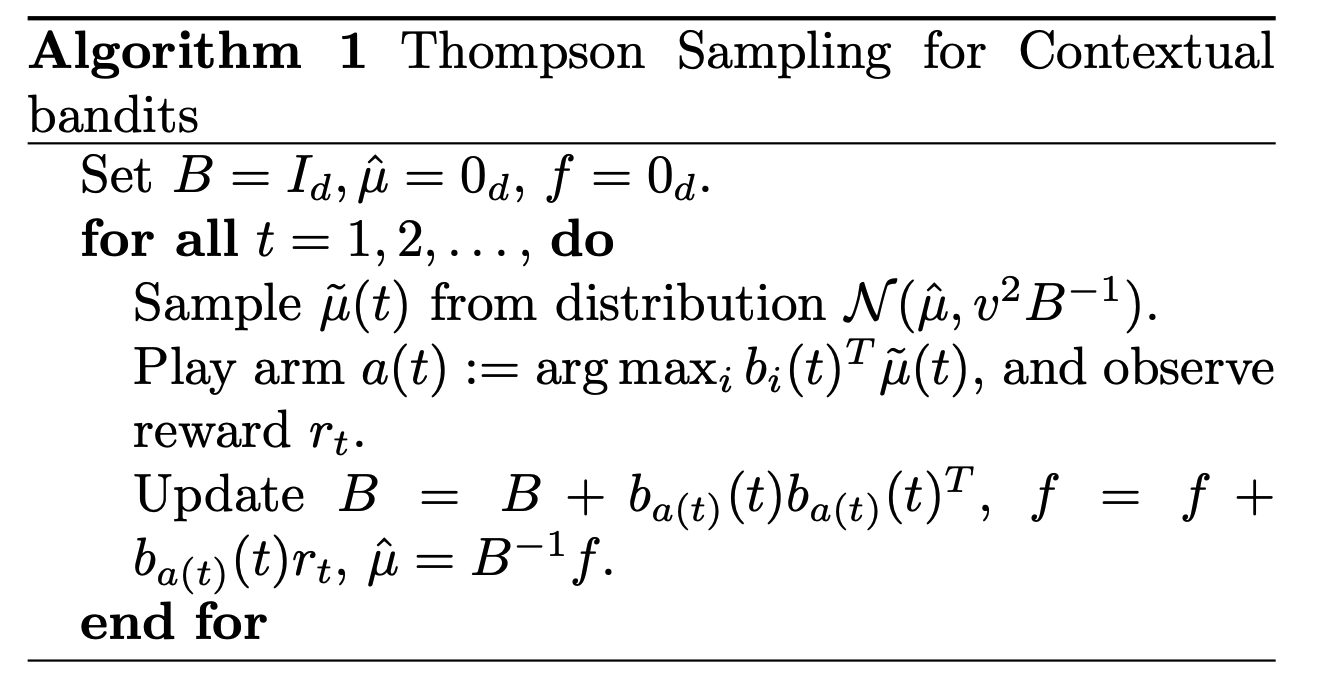
\includegraphics[width=.5\linewidth]{images/thompson_sampling_algorithm.png}
  \caption{Definition of the Thompson sampling algorithm taken from \href{http://proceedings.mlr.press/v28/agrawal13.pdf}{paper}}
\end{figure}

Run the Thompson Sampling algorithm with the following command:

\begin{lstlisting}
$ python run.py --model thompson
\end{lstlisting}

You should see the total\_fraction\_correct to be \textbf{around} 0.64, though the results may vary per run.

\textit{Note: please feel free to adjust the --v2 argument, but you don't have to. This is actually v squared from the paper) }